\section{Polynomial Modeling}\label{sec:pmodel} 

\begin{figure*}[hbt]
    \begin{center}
    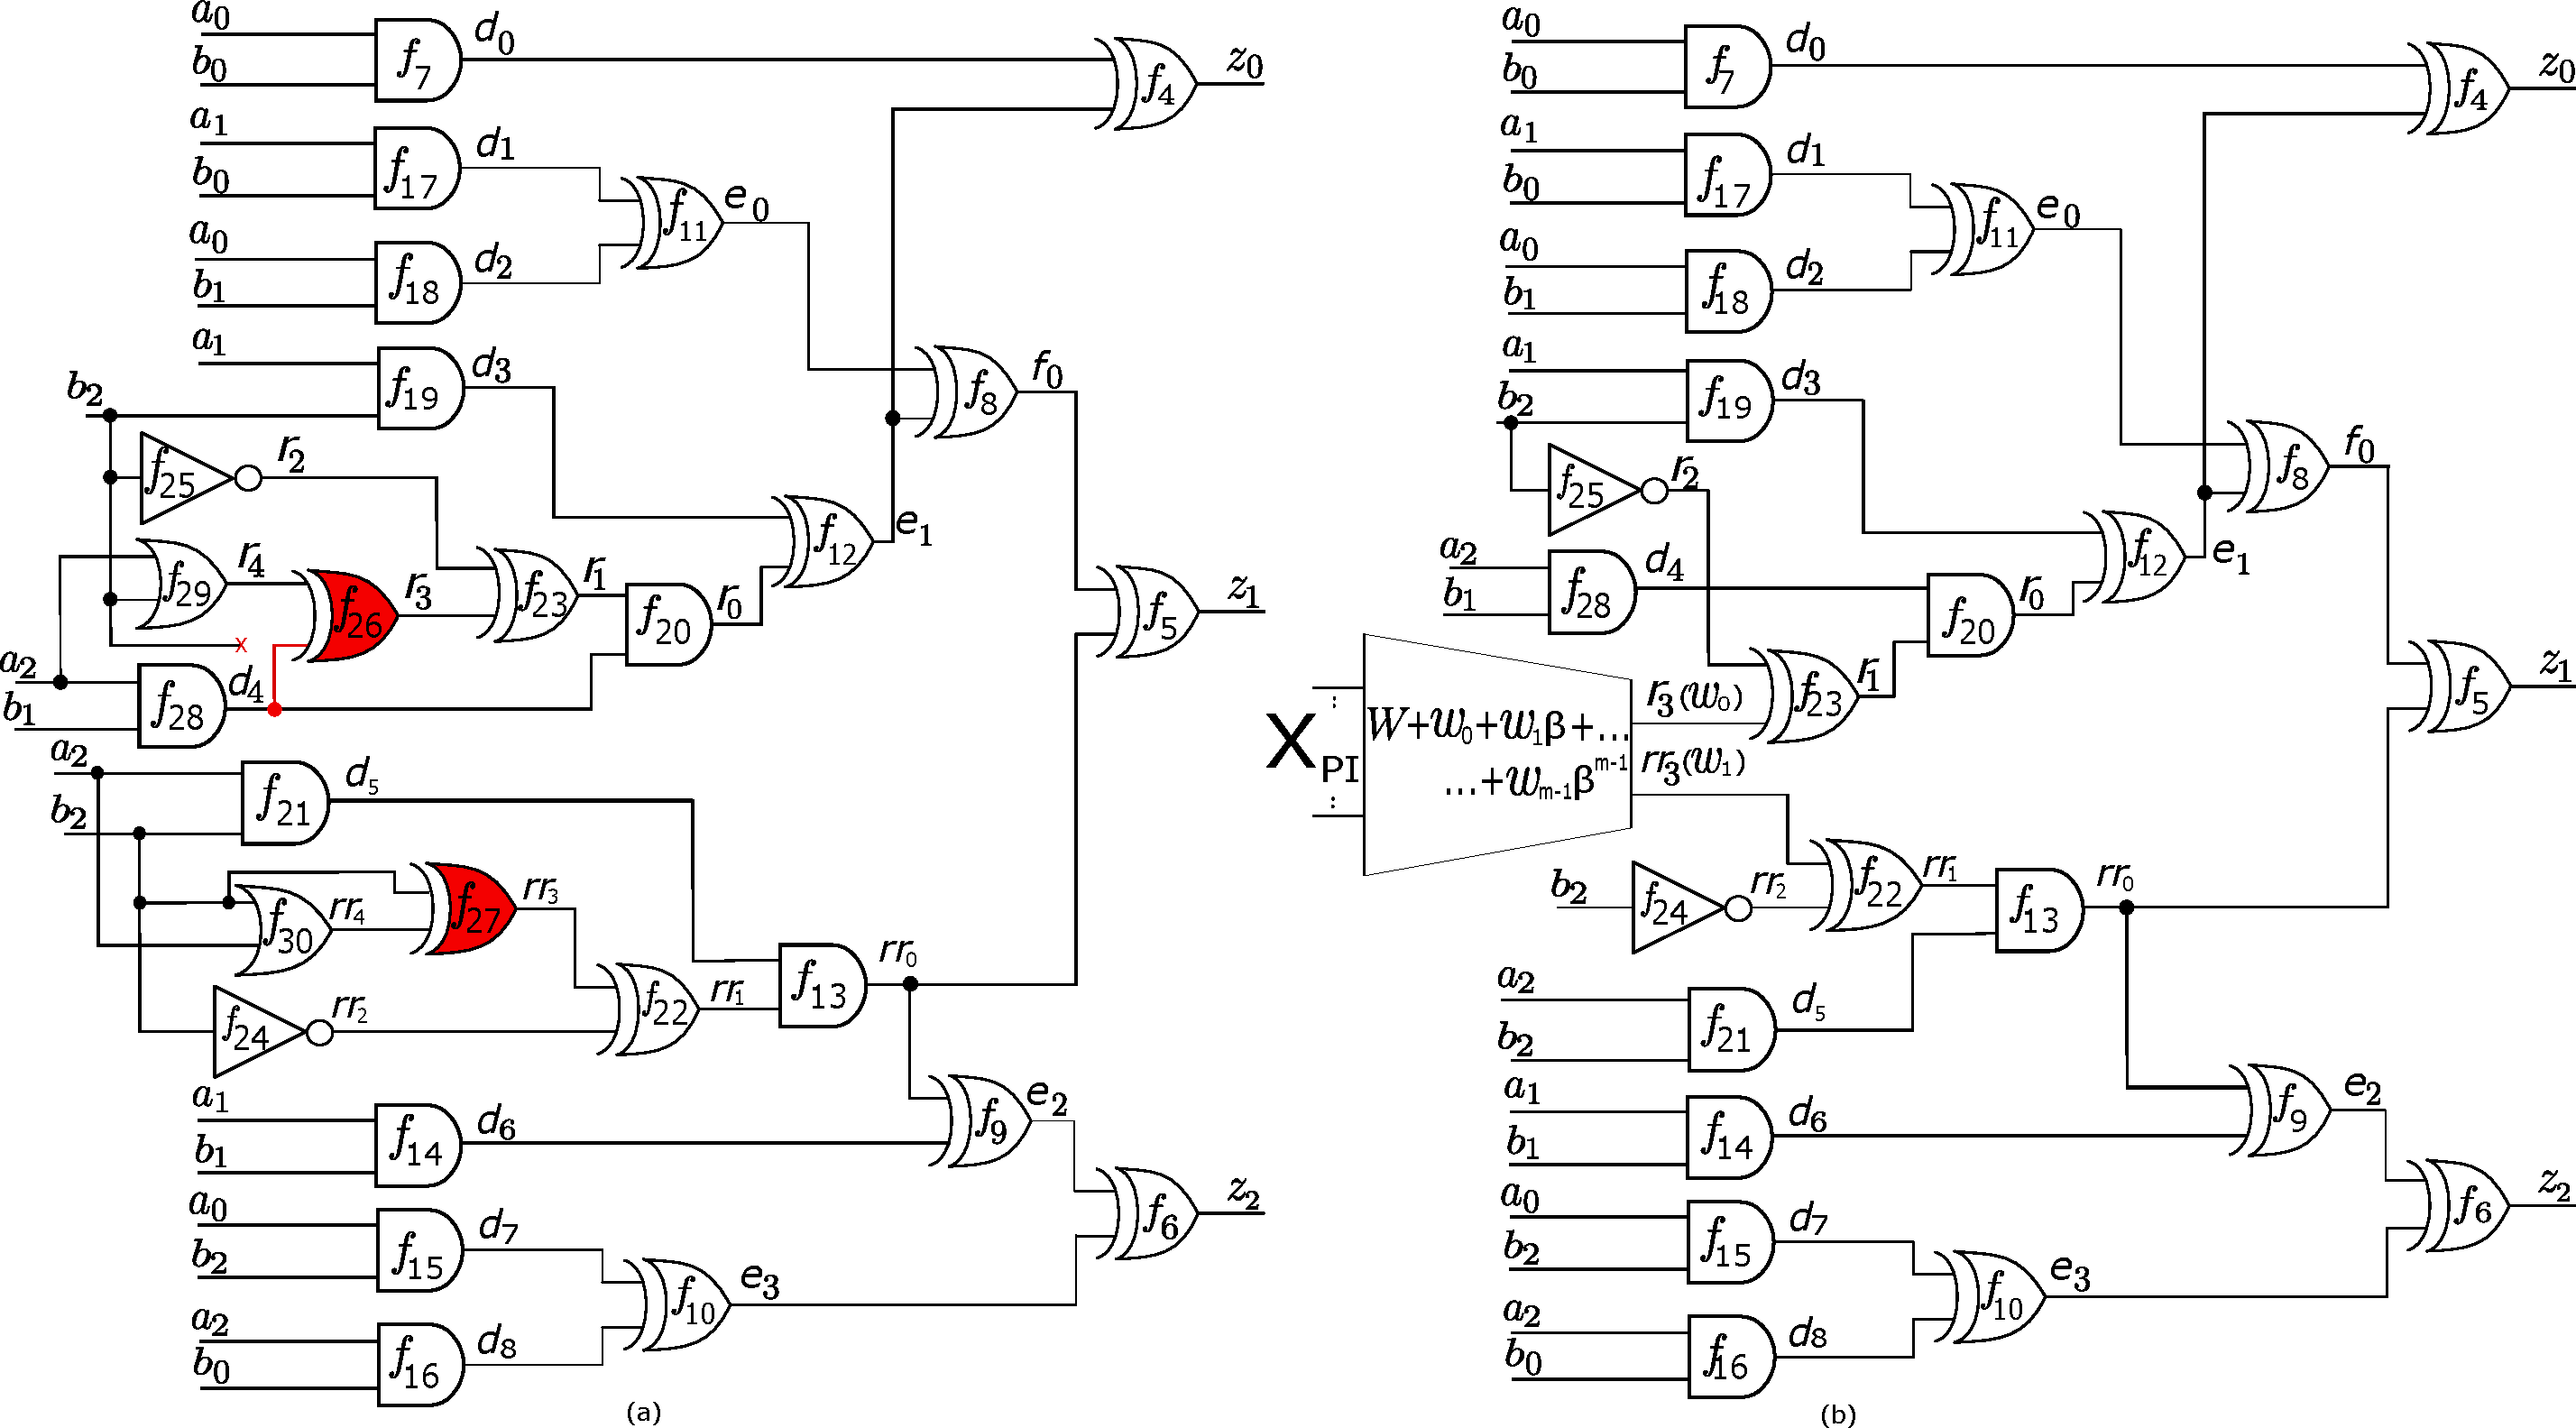
\includegraphics[scale = 0.31]{mas_3_ddc_mfr.pdf}
    \end{center}
    \caption{{\footnotesize  
    (a) A buggy implementation of a 3-bit finite field multiplier ($n$=3)
    with bugs introduced at net $r_3$ (AND gate replaced with an XOR
    gate and one of the inputs misconnected to $d_4$ instead of $b_2$)
    and net $rr_3$ (AND replaced with an XOR) (b) Patch function
    modeled as a 2-bit-vector word ($m$=2), $f_W: W+r_3+\be \cdot rr_3$
    ($w_0=r_3, w_1=rr_3$).} }
    \label{fig:mas_bug_W}\vspace{-0.25in}
\end{figure*}

% Rectification begins after verification detects the presence of bugs
% in the design. 
% For verification of finite field arithmetic circuits,
% the approach based on \cite{lv:tcad2013} has been shown to be 
% successful. As the algebraic setup for verification is augmented
% for subsequent rectification, we review the main concepts from
% \cite{lv:tcad2013} below. 
% The algebraic setup used in our MFR checking procedure 
% We perform verification using the approach presented in~\cite{lv:tcad2013}. 
% , utilize the same setup as a starting point for MFR checking. 
% We review the main concepts from~\cite{lv:tcad2013} below:

% We use an augmentation of the algebraic setup presented in~\cite{lv:tcad2013}
% as a starting point for the MFR checking procedure. We therefore review the 
% main concepts and verification setup from~\cite{lv:tcad2013} below:

A multivariate polynomial $f$ with coefficients in a finite field
$\Fkn$ is given as a specification, where $n$ is the operand
word-length (datapath size). A corresponding combinational
circuit $C$ is given as its implementation. 
The function implemented by the circuit $C$ is modeled with a system of polynomials over 
$R=\Fkn[Z,A,x_1,\dots,x_d]$. Here $\{x_1, \dots$ $, x_d\}$ correspond 
to all the bit-level variables (nets) in the circuit, and $Z,A$ the 
output and input words, respectively.  The field $\Fkn$ is constructed
as $\Fkn = \Ftwo[X]\pmod{P_n(X)}$, where $P_n(X)$ is the given
primitive polynomial of degree $n$
with $\ga$ as a root, i.e. $P_n(\ga) =0$. 
As $C$ comprises Boolean logic gates, they are
mapped to polynomial functions over $\F_2 (\subset \Fkn) \pmod 2$: 
% as follows: 
\vspace{-0.15in}

\begin{small} 
\begin{equation}
\label{bool2poly}
\begin{split}
z =  \neg a \mapsto z+a+1;~~~& z =  a \wedge b \mapsto z+a \cdot b;\\
z =  a \vee b \mapsto z+a+b+a \cdot b;~~~& z =  a \oplus b \mapsto z+a+b;
\end{split}
\end{equation}
\end{small}
% \begin{small} 
% \begin{equation}
% \label{bool2poly}
% \begin{split}
% z =  \neg a &\rightarrow z+a+1 \pmod 2  \\
% z =  a \wedge b &\rightarrow z+a \cdot b \pmod 2\\
% z =  a \vee b &\rightarrow z+a+b+a \cdot b \pmod 2 \\
% z =  a \oplus b &\rightarrow z+a+b \pmod 2 
% \end{split}
% \end{equation}
% \end{small}
\vspace{-0.15in}

Similarly, the primary output and input bits $z_i, a_i: i=0,\dots,n-1$ 
can be correlated to the corresponding operand words $Z,A$ as follows:
\vspace{-0.08in}
\begin{equation}
\label{ip-word-level}
\begin{split}
 f_1: Z + z_0 +\gamma \cdot  z_1 + \dots +\gamma^{n-1} \cdot z_{n-1}\\
 f_2: A + a_0 +\gamma \cdot a_1 + \dots +\gamma^{n-1} \cdot a_{n-1}
\end{split}
\end{equation}

% where $\gamma$ is a PE of $\Fkn$. 
Thus, the circuit is represented
by a set of polynomials $F=\{f_1,\dots,f_s\} \subset
R$. Let $J =\langle F\rangle$ be the ideal
generated by this set.
%Let $X_{PI} \subset \{x_1,\dots,x_d\}$ be the primary input variables
%of the circuit. Let $F_0^{PI}=\{x_i^2-x_i:x_i\in X_{PI}\}$ denote the
%set of bit-level vanishing polynomials in primaryinputs, and let $J_0
%= \langle F_0^{PI} \rangle$ be the ideal of vanishing polynomials.
Let $F_0 = \{x_i^2-x_i, Y^{2^n}-Y: x_i \in \text{bit-level variables},
Y \in \text{word-level variables}\}$ be the set of all vanishing
polynomials, and $J_0 = \langle F_0\rangle$ be the corresponding ideal. 

While it is assumed that the given circuit $C$ is buggy, it is important 
to note that the verification test can be formulated as {\textit{ideal
membership  testing}} of $f$ in $J+J_0$ using
GB~\cite{lv:tcad2013}, i.e. by  
checking if $f\xrightarrow{GB(J+J_0)}_+0$.
It has now become standard practice to impose {\it Reverse Topological Term Order (RTTO)} to 
overcome the complexity of GB computations, which ensures the set of
polynomials $F\cup F_0$ itself constitute a GB of $J+J_0$. This simplifies
the above {\textit{ideal membership testing}} to that of checking if the polynomial division
$f\xrightarrow{F+F_{0}}_+0$.
% . When $C$ correctly implements $f$, then $f$ agrees
% with every evaluation of all the nets in $C$. In other words, $f$
% vanishes on $V(J)$, or equivalent{}ly $f \in I(V(J))$. The Strong
% Nullstellensatz in finite fields (Thm. \ref{thm:strong-ns}) tells us
% %Nullstellensatz in finite fields tells us
% that $I(V(J)) = J + J_0$, where $J_0 = \langle F_0 \rangle = \langle x_1^2-x_1,\dots
% ,x_d^2-x_d,Z^{2^n}-Z, A^{2^n}-A\rangle$. Thus, the verification test can be formulated as
% ideal membership testing of $f$ in $J+J_0$ using \Grobner bases: We will
% check if $f\xrightarrow{GB(J+J_0)}_+0$?
% Further, the authors~\cite{lv:tcad2013} impose a specialized term order
% '$>$` called the {\it Reverse Topological Term Order (RTTO)} on the
% polynomials. RTTO is derived by ordering the nets (variables) of $C$
% in reverse topological order from primary outputs to primary inputs,
% and imposing a {\it lex} order on the monomials. It has
% now become standard practice to utilize RTTO-style term orders to 
% overcome the complexity of GB computations.
% RTTO $>$ ensures
% that each net at a gates output appears as a leading term of some
% polynomial in $F$. 
% As each gate output is a distinct net, the
% leading terms of all polynomials in $F$ become relatively
% prime. Thm. 6.1 and Cor. 6.1 in \cite{lv:tcad2013} show that due to
% the above characteristics, {\it RTTO $>$ renders the set of
%   polynomials $F\cup F_0$ itself a GB of $J+J_0$.}
%As the set $F\cup F_0$ is a GB is itself,
% As a result, the expensive GB computation is avoided altogether, and
% the verification check reduces to that of polynomial division
% $f\xrightarrow{F,F_{0}}_+r$, and checking whether $r=0$.
In the sequel, we use the circuit shown in
Fig. \ref{fig:mas_bug_W} as a running example to demonstrate our
approach for MFR. 

\begin{Example}
\label{verify_ex}
The circuit $C$ in Fig. \ref{fig:mas_bug_W} (a) is a buggy
implementation of a 3-bit ($n$=3) Mastrovito multiplier. 
The field $\F_{2^3}$ is constructed using $P_3(X)=X^3+X+1$
and let $\ga$ be a PE of $\F_{2^3}$, s.t. $P_3(\ga)=0$. The \spec ~polynomial is $f: Z + A\cdot B$, where
$Z$ is the output word, and $A,B$ the input words. RTTO $>$ is derived
to be a {\it lex} term order with variable order: 
\begin{small}
% $\{Z\}>\{A>B\}>\{z_0>z_1>z_2\}>\{d_0>f_0>e_2>e_3\}>\{e_0>e_1>rr_0>d_6>d_7>d_8\}>\{d_1>d_2>d_3>r_0>d_5>rr_1\}>\{r_1>rr_3>rr_2\}>\{r_2>r_3>rr_4\}>\{r_4>d_4\}>\{a_0>a_1>a_2>b_0>b_1>b_2\}$
$\{Z\}>\{A>B\}>\{z_0>z_1>z_2\}>\cdots>\{d_1>d_2>d_3>r_0>d_5>rr_1\}>\{r_1>rr_3>rr_2\}>\{r_2>r_3>rr_4\}>\{r_4>d_4\}>\{a_0>a_1>a_2>b_0>b_1>b_2\}$.
\end{small}

The following polynomials represent the function implemented by $C$,
with terms ordered according to RTTO $>$.
% {\small\begin{flalign*}
% f_1:Z + z_0 +\ga z_1 + \ga^2 z_2;  	&\quad f_{16}:d_8 + a_2b_0; \\
% f_2:A + a_0 +\ga a_1 + \ga^2 a_2;  	&\quad f_{17}:d_1 + a_1b_0; \\
% f_3:B + b_0 +\ga b_1 + \ga^2 b_2;  	&\quad f_{18}:d_2 + a_0b_1; \\
% f_4:z_0 + d_0 + e_1;               	&\quad f_{19}:d_3 + a_1b_2; \\
% f_5:z_1 + f_0 + rr_0;             	&\quad f_{20}:r_0 + r_1d_4; \\
% f_6:z_2 + e_2 + e_3;			   	&\quad f_{21}:d_5 + a_2b_2; \\
% f_7:d_0 + a_0b_0;                  	&\quad f_{22}:rr_1 + rr_2+rr_3; \\
% f_8:f_0 + e_0 + e_1;               	&\quad f_{23}:r_1 + r_2+r_3; \\
% f_9:e_2 + rr_0 + d_6;              	&\quad f_{24}:rr_2 + b_2 + 1; \\ 
% f_{10}:e_3 + d_7 + d_8;            	&\quad f_{25}:r_2 + b_2 + 1; \\
% f_{11}:e_0 + d_1 + d_2;      	   	&\quad \red{f_{26}:r_3 + d_4 + r_4;}\\
% f_{12}:e_1 + d_3 + r_0;				&\quad \red{f_{27}:rr_3 + rr_4 + b_2;} \\
% f_{13}:rr_0 + d_5rr_1;			    &\quad f_{28}:d_4 + a_2b_1; \\
% f_{14}:d_6 + a_1b_1;				&\quad f_{29}:r_4 + a_2 + b_2 + a_2b_2; \\
% f_{15}:d_7 + a_0b_2;				&\quad f_{30}:rr_4 + a_2 + b_2 + a_2b_2; \\
% \end{flalign*}}
% \vspace{-0.1in}
% \begin{small}
% \begin{flalign*}
% f_1:Z + z_0 +\ga z_1 + \ga^2 z_2;  	&\quad \dots\\
% f_2:A + a_0 +\ga a_1 + \ga^2 a_2;  	&\quad f_{22}:rr_1 + rr_2+rr_3; \\
% f_3:B + b_0 +\ga b_1 + \ga^2 b_2;  	&\quad f_{23}:r_1 + r_2+r_3; \\
% f_4:z_0 + d_0 + e_1;               	&\quad f_{24}:rr_2 + b_2 + 1; \\ 
% f_5:z_1 + f_0 + rr_0;             	&\quad f_{25}:r_2 + b_2 + 1; \\
% f_6:z_2 + e_2 + e_3;			   	&\quad \red{f_{26}:r_3 + d_4 + r_4;}\\
% f_7:d_0 + a_0b_0;					&\quad \red{f_{27}:rr_3 + rr_4 + b_2;} \\
% f_8:f_0 + e_0 + e_1;				&\quad f_{28}:d_4 + a_2b_1; \\
% f_9:e_2 + rr_0 + d_6;             	&\quad f_{29}:r_4 + a_2 + b_2 + a_2b_2; \\
% \dots								&\quad f_{30}:rr_4 + a_2 + b_2 + a_2b_2;
% \end{flalign*}
% \end{small}
\begin{small}
\begin{flalign*}
\vspace{0.4in}
f_1:Z + z_0 +\ga \cdot z_1 + \ga^2 \cdot z_2;   &\quad f_{22}:rr_1 + rr_3+rr_2; \\
f_2:A + a_0 +\ga \cdot a_1 + \ga^2 \cdot a_2;   &\quad f_{23}:r_1 + r_2+r_3; \\
f_3:B + b_0 +\ga \cdot b_1 + \ga^2 \cdot b_2;   &\quad \red{f_{26}:r_3 + r_4 + d_4;}\\
f_4:z_0 + d_0 + e_1;                &\quad {\red f_{27}:rr_3 + rr_4 + b_2;} \dots\\
\dots                               &\quad f_{30}:rr_4 + a_2+b_2+a_2b_2;
\end{flalign*}
\end{small}
\vspace{-0.2in}
% \begin{small}
% \begin{flalign*}
%                                     &\quad \dots\\
% \dots                               &\quad f_{30}:rr_4 + a_2+b_2+a_2b_2;
% \end{flalign*}
% \end{small}
% \vspace{-0.2in}

% \vspace{-0.1in}
% \begin{small}
% \begin{flalign*}
% f_1:Z + z_0 +\ga z_1 + \ga^2 z_2;   &\quad f_{22}:rr_1 + rr_2+rr_3; \\
% f_2:A + a_0 +\ga a_1 + \ga^2 a_2;   &\quad f_{23}:r_1 + r_2+r_3; \\
% f_3:B + b_0 +\ga b_1 + \ga^2 b_2;   &\quad \dots\\ 
% f_4:z_0 + d_0 + e_1;                &\quad \red{f_{26}:r_3 + d_4 + r_4;}\\
%                                     &\quad \red{f_{27}:rr_3 + rr_4 + b_2;} \\
%                                     &\quad \dots\\
% \dots                               &\quad f_{30}:rr_4 + a_2 + b_2 + a_2b_2;
% \end{flalign*}
% \end{small}
% The correct circuit will have polynomials $f_{10},f_{12},$ and $f_{18}$ above replaced by 
% $f_{10_c} = e_0 + d_1 + d_2, f_{12_c}:d_5 + a_2b_2,$ and  $f_{18_c}:d_2 + a_2b_1$ respectively.
Then $F = \{f_1,\dots,f_{30}\}$, $F_0 =
\{a_0^2-a_0,\dots,z_2^2-z_2,A^8-A,B^8-B,Z^8-Z\}$, and under RTTO $>$, $F\cup
F_{0}$ constitutes a GB of $J+J_0=\langle F\cup F_0\rangle$.
% Computing $f: Z + A\cdot  B\xrightarrow{F,F_{0}}_+r$ results in $r =
%  \ga^2(a_1a_2b_1b_2+a_1a_2b_2+a_2b_1b_2) +
%  \ga^1(a_1a_2b_1b_2+a_1a_2b_2) + \ga^0(a_2b_1b_2)$. Since  $r\neq 0$,
%  the circuit is buggy.  
\end{Example}
% Our objective now is to identify a set of $m$-target nets where MFR can be
% performed, confirm the existence of a rectification function at these nets, 
% and then to subsequently compute a rectification function. 
%% Note that we can also formulate equivalence
%% verification between a specification $C_s$ and a buggy implementation $C_i$,
%% both given as gate level circuits. The verification problem is modeled as 
%% a word-level miter, with the inputs of $C_s$ and $C_i$ connected together. 
%% Let $Z_{s}$ and $Z_{i}$ represent the word-level outputs of $C_s$ and $C_i$,
%% respectively. With $C_s$ and $C_i$ modeled as polynomial ideals (under RTTO $>$) 
%% $F_s$ and $F_i$, respectively, we formulate the verification problem 
%% as $Z_s-Z_i\xrightarrow{F_s,F_i,F_{0}^{PI}}_+r$, and by checking whether $r=0$?. 
% identifying rectification targets is not clear.
% algorithmically where do you place W? need to formalized and written under net picking W.
% what are the functions that our approach is building?

Since $\F_2 \subset \Fkn$, the polynomials in Eqn. (\ref{bool2poly}) can also 
be interpreted as polynomials over $\Fkn$. The advantage of working over the 
field $\Fkn$ is that we can represent and manipulate both the bit-level
and $n$-bit word-level polynomials in one unified domain. However, we are 
given a patch word-length $m$ which is modeled as an $m$-bit-vector word over field $\Fkm$. 
Since the field $\Fkm$ might not be compatible with the field $\Fkn$, not every $m$-bit-vector 
can be construed as an element in $\Fkn$. 
To overcome this incompatibility, the following section presents techniques which help 
model polynomial operations in a unified domain.

\vspace{-0.12in}